\chapter{Development components}
\label{ch:development-components}

\section{Development workflow}
\label{sec:development-workflow}


\begin{figure}
\centering
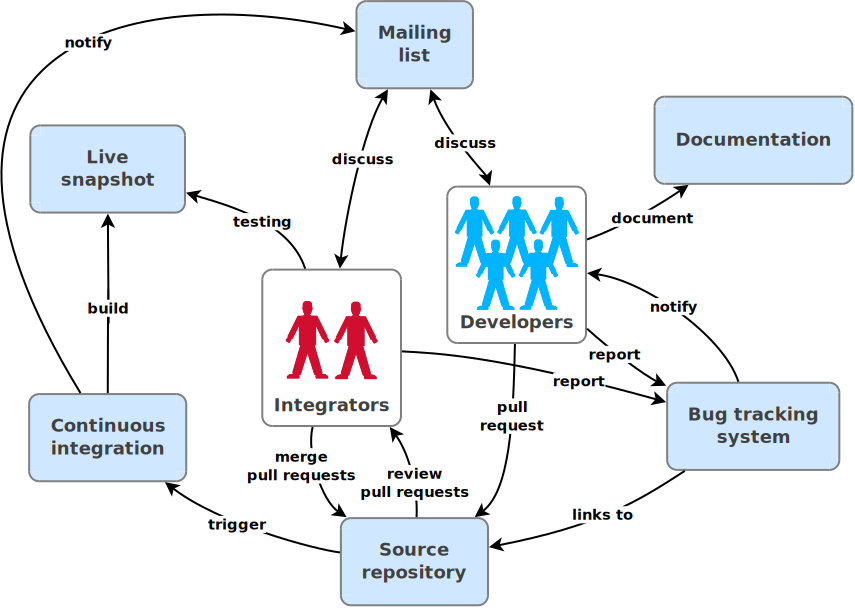
\includegraphics[width=0.67\textwidth]{images/development-workflow.png}
\caption{Development workflow with all tools}
\label{fig:development-worflow}
\end{figure}
[[image:Workflow.png||width="60%"]]

\section{Details}
\label{sec:details}

The previous figure illustrates the global development workflow.  In this workflow, there is two different kind of actors (developers and committers) which interact with different kind of tools.  We will now give more details on these tools and how they will be used by the actors.

\subsection{Mailing list}
\label{sec:mailing-list}

Most of the communication between the developers and the committers use the mailing list medium to interact and discuss general decision about the platform.  The goal is to keep traces of any discussion or choice that may have been made about developments or architecture design.

\subsection{Source repository}
\label{sec:source-repository}

This is where every part of source code or binary for building the LearnPAd platform are stored.  Only a subset of people, the committers, have the rights to modify and update this repository.  Developers propose new functionality or bug fixing as pull requests that committers will review then will accept or reject.  Every pull request should link to the corresponding bug (in the bug tracking system) when it applies.

\subsection{Documentation}
\label{sec:documentation}

Developers document what they are developing on a centralized tool.  On this tool, they push source documentation, architecture documentation, interface and API documentation.

\subsection{Bug tracking system}
\label{sec:bug tracking-system}

Committers may detect bugs during the reviewing step; they will report them on the bug tracking system which in return will notify concerned developers.  Developers are also using the bug tracking system to report and trace bugs.  For the reporting, links with the source repository must be done (a version, a file, a component, etc.).

\subsection{Continuous integration}
\label{sec:continuous-integration}

The goal of continuous integration is to regularly check that everything published on the source repository is always buildable and meets at least major functionalities.  He also automatically check the last version against pull request to help committers to take decisions about a pull request; as long as a pull request imply a wrong build of the platform, it must be rejected.

\subsection{Live snapshot}
\label{sec:live-snapshot}

Live snapshots are the result of the continuous integration building the LearnPAd platform against each of the opened pull requests.  The committers use these snapshots to test and review pull requests before accepting them.
